\documentclass{ieeeaccess}
\usepackage{cite}
\usepackage{amsmath,amssymb,amsfonts,siunitx,multirow,booktabs,dcolumn}
\usepackage{algorithmic}
\usepackage{graphicx}
\usepackage{textcomp}
\usepackage{multirow}
\def\BibTeX{{\rm B\kern-.05em{\sc i\kern-.025em b}\kern-.08em
    T\kern-.1667em\lower.7ex\hbox{E}\kern-.125emX}}
\begin{document}
\history{Received September 8, 2018, accepted September 28, 2018, date of publication October 10, 2018,\\
date of current version November 8, 2018.}
\doi{10.1109/ACCESS.2018.2875135}

\title{Key Concept Identification: A Sentence Parse
Tree-Based Technique for Candidate Feature
Extraction From Unstructured Texts}

\author{\uppercase{MUHAMMAD AMAN}\authorrefmark{1}, \uppercase{ABAS BIN MD SAID}\authorrefmark{1}, \uppercase{SAID JADID ABDUL KADIR}\authorrefmark{1}, \\
\uppercase{AND ISRAR ULLAH}\authorrefmark{2}}

\address[1]{Department of Computer and Information Sciences, Universiti Teknologi Petronas, Seri Iskandar 32610, Malaysia}
\address[2]{Computer Engineering Department, Jeju National University, Jeju 63243, South Korea}

\tfootnote{This work was supported by Universiti Teknologi Petronas, Malaysia.}

\markboth
{M. Aman \headeretal:  Key Concept Identification: A Sentence Parse Tree-Based Technique for Candidate Feature Extraction}
{M. Aman  \headeretal:  Key Concept Identification: A Sentence Parse Tree-Based Technique for Candidate Feature Extraction}

\corresp{Corresponding author: Muhammad Aman (muhammad.aman\_g03419@utp.edu.my)}

\begin{abstract}
The effectiveness of automatic key concept or keyphrase identification from unstructured text documents mainly depends on a comprehensive and meaningful list of candidate features extracted from the documents. However, the conventional  techniques for candidate feature extraction limit the performance of keyphrase identification algorithms and need  improvement. The objective of this paper is to propose a novel parse tree-based approach for candidate feature extraction to overcome the shortcomings of the existing techniques. Our proposed technique is based on generating a parse tree for  each sentence in the input text. Sentence parse  trees are then cut into sub-trees to extract branches for candidate  phrases (i.e., noun, verb, and so on). The sub-trees are  combined using parts-of-speech tagging to generate the flat  list of candidate phrases. Finally, filtering is performed using heuristic rules and redundant phrases are eliminated to  generate final list of candidate features. Experimental analysis is conducted for validation of the proposed scheme using three manually annotated and publicly available data sets from different domains, i.e., Inspec, 500N-KPCrowed, and SemEval-2010. The proposed technique is fine-tuned to determine the optimal value for the parameter context window size and then it is compared with the existing conventional n-gram and noun-phrase-based techniques. The results show that the proposed technique outperforms the existing approaches and significant improvements of 13.51\% and 30.67\%, 12.86\% and 5.48\%,  and 13.16\% and 31.46\% are achieved, in terms of \textit{precision, recall}, and \textit{F-measure} when compared with noun-phrasebased  scheme and n-gram-based scheme, respectively. These results give us confidence to further validate the proposed technique by developing a keyphrase extraction algorithm in the future.
\end{abstract}

\begin{keywords}
Keyphrase extraction, feature extraction, key concept extraction, information retrieval, text mining.
\end{keywords}

\titlepgskip=-15pt

\maketitle

\section{Introduction}
\label{sec:introduction}
Automatic keyphrase identification is a challenging problem in many application areas such as text mining, document  categorization and summarization, information retrieval and proposed in the literature to address this problem that can be broadly categorized into two classes (i.e. supervised and un-supervised approaches). Candidate feature selection is a fundamental task in every proposed solution, and thus the efficiency and robustness of the methods mainly depend on the  underlying candidate feature extraction technique. A comprehensive and syntactically correct list of candidate feature may ensure a robust set of keyphrases. 

Conventionally, n-gram or noun-phrase based techniques are used for candidate feature extraction. However, the existing  approaches have certain limitations which make it difficult to obtain a comprehensive list of candidate phrases. One  problem in the n-gram based approach is that, the length of n-grams is restricted; secondly, the candidate phrases are  most likely incorrect grammatically, besides they do not always capture complete information \cite{b1}. Similarly, the noun  phrases, which can be a single noun or group of words that work as a noun, have the problem that not all nouns are  keyphrases and conversely, there might be phrases other than nouns that are potentially keyphrases or part of a  keyphrase. For instanse, in the key concept ‘extracting concepts,’ the ‘extracting’ is a verb with type verb gerund (VBG) not noun (NN), however, potentially it is similar to the concept of ‘concept extraction’. The same way, when the  keyphrase ‘distributed computing’ is parsed, the word ‘distributed’ was tagged as VBN, that is verb. So, if we use the  linguistic pattern \textit{(Adjective)*(noun)+} to find noun phrases as candidates, then many important key concepts, like the ones mentioned in the previous example, might be missed.

We assume that  creating a parse tree of a sentence depicts a complete picture of the sentence. It shows the overall  structure and the relationship between various parts of the sentence. For instance, the parse tree of the lengthy  sentence \textit{‘‘The strongest rain ever recorded in India shut down the financial hub of Mumbai, snapped communication lines,  closed airports and forced thousands of people to sleep in their offices or walk home during the night, officials said today’’} \cite{b2} is given in Figure \ref{fig:f1}, which not only shows the POS tags of words but interlinks various parts of the sentence. So, analyzing a sentence parse tree and extracting meaningful candidate phrases based on parsing technique is  more effective compared to relying only on POS tagging and linguistic patterns.
    
Furthermore, after the analysis of a sentence  structure, it can be classified as simple, compound or complex sentence. A simple sentence consists of one clause, where clause in English has at least two parts, i.e., noun phrase and verb phrase. A compound sentence has two or more clauses joined by coordinating conjunctions, while a complex sentence has one main clause and one or more adverbial clauses joined by subordinating conjunctions \cite{b3}. Therefore, the basic unit of a  sentence that gives a complete information about a key concept can be a clause structure. Most clauses consist of a noun  phrase, verb phrase and prepositional phrase. So,  we assume that for effective candidate feature extraction all of the  three kinds of phrases should be considered simultaneously instead of noun phrases alone, and the task can be best  accomplished by analyzing a sentence in the form of a parse tree structure. 
		
Based on the rationale discussed above, we developed a novel parsing-based technique for candidate feature extraction.  This research contributes by
\begin{itemize}	
	\item Introducing a new approach that significantly improves candidate feature extraction from unstructured text for key concepts identification.
	\item Providing a method for extracting contextual information as a part of candidate features, that can be utilized for semantic based information retrieval.
\end{itemize}

\Figure[!h] ()[width=0.75\linewidth]{fig1.png}{\textbf{Example of sentence parse tree and candidate features
extraction.\label{fig:f1}}}

The rest of the paper is organized as follows: Section II presents the related studies on candidate feature extraction. The proposed technique is described in details in Section III. In section IV we present the details of the experiments conducted and discuss the results. Section V concludes the paper with future work recommendation.

\section{RELATED WORK}
Candidate feature extraction is a common task in almost all approaches for key concepts identification and most of them rely on the two conventional techniques in this regard (i.e. n-gram based, and noun phrases-based However, as discussed  in section I, the problem with the n-gram approach is that the length of n-grams is restricted. Furthermore, n-grams are  most likely incorrect grammatically and do not always capture complete information \cite{b1}. An alternative solution to  this problem is the use of certain linguistic patterns based on part-of-speech (POS) tags or noun phrases \cite{b1}, \cite{b10}–\cite{b16}. These techniques follow Hulth observation that most keyphrases are noun phrases \cite{b17}. The first preprocessing step in these algorithms consists of part-of-speech (POS) tagging, which provides tags to each individual  word in a sentence and makes it easy to retrieve noun phrases as candidate features. Nevertheless, not all nouns are keyphrases and there might be phrases other than nouns that are potentially keyphrases or part of a keyphrase. Also, it  is hard to find linguistic patterns that cover all the key concepts. Although a majority of the approaches depend on the  above two techniques for candidate features extraction, some other solutions have been proposed for the subtask. Boudin  and Morin \cite{b18} use a multi-sentence compression approach based on word graph \cite{b19}, \cite{b20}, to obtain the initial candidate features, that is,s what they have called compression candidates. This approach constructs a directed word graph from a set of input sentences. The nodes in the graph represent the unique words and the edges show the structure of the original sentences (i.e. word sequence). The common paths in the graph are used to obtain the   compression candidates. Another approach for candidate features extraction is based on word expansion \cite{b21}. This  approach first generates a set of core words to find out competitive positions for potential keyphrases. After that a  technique based on core word expansion trees is used to produce candidate features from these positions. The technique  ensures that a maximum of two candidates are generated from each occurrence of the core word. Some others have used  heuristic approaches \cite{b22}, \cite{b23}.
 
Wang \headeretal  \cite{b24} and Zheng \headeretal  \cite{b25} utilize description knowledge for keyphrase extraction and select candidate phrases with respect to Wikipedia using Wikipedia Miner for mapping between the given document and Wikipedia entities. 

Bennani-Smires \headeretal \hspace{0.75 mm} recently developed a technique which is also based on the noun phrase approach using linguistic patterns of POS tags \cite{b26}. It selects those phrases that consist of zero or more adjectives and followed by one or more nouns.

Some other recent works aim at exploiting keyword extraction for text classification. Wu \headeretal \cite{b27} proposed a probabilistic approach for keyword extraction that is inspired by visual attention mechanism. Individual words are  considered as candidate features which are further assigned probability-based scores. Hu \headeretal have used  distributed representation of words in extracting keywords for patent classification \cite{b28}. In this approach words  are used as candidate features which are assigned rank based on cosine similarity of the candidate word with the centroid word of the given document. To overcome the shortcomings of the existing conventional approaches, we propose a novel  technique for candidate feature extraction based on sentence parsing. In the next section we describe the proposed technique in detail.

\Figure[!h] ()[width=0.9\linewidth]{fig2.png}{\textbf{Block Diagram of Proposed Technique for Candidate Features
Extraction.\label{fig:f2}}}

\begin{table*}[!h]
\centering
\caption{\textbf{Description of part-of-speech (POS) tags \cite{b30}.}}
\label{tab:t1}
\begin{tabular}{|r|l|l|r|l|l|} 
\hline
S.No. & POS Tag & Description                              & S.No. & POS Tag & Description                                   \\ 
\hline
1     & CC      & Coordinating conjuction                  & 19    & PRPS    & Possessive pronoun (prolong version PRP-S)~   \\ 
\hline
2     & CD      & Cardinal number                          & 20    & RB      & Adverb                                        \\ 
\hline
3     & DT      & Determiner                               & 21    & RBR     & Adverb, comparative                           \\ 
\hline
4     & EX      & Existential there                        & 22    & RBS     & Adverb, superlative                           \\ 
\hline
5     & FW      & Foreign word                             & 23    & RP      & Particle                                      \\ 
\hline
6     & IN      & Preposition or subordinating conjunction & 24    & SYM     & Symbol                                        \\ 
\hline
7     & JJ      & Adjectve                                 & 25    & TO      & to                                            \\ 
\hline
8     & JJR     & Adjective, comparative                   & 26    & UH      & Interjection                                  \\ 
\hline
9     & JJS     & Adjective, superlative                   & 27    & VB      & Verb, base form                               \\ 
\hline
10    & LS      & List item marker                         & 28    & VBD     & Verb, past tense                              \\ 
\hline
11    & MD      & Modal                                    & 29    & VBG     & Verb, gerund or present participle            \\ 
\hline
12    & NN      & Noun, singular or mass                   & 30    & VBN     & Verb, past participle                         \\ 
\hline
13    & NNS     & Noun, plural                             & 31    & VBP     & VErb, non 3rd person singular present         \\ 
\hline
14    & NNP     & Proper noun, singular                    & 32    & VBZ     & Verb, 3rd person singular present             \\ 
\hline
15    & NNPS    & Proper noun, plural                      & 33    & WDT     & Wh-determiner                                 \\ 
\hline
16    & PDT     & Predeterminer                            & 34    & WP      & Wh-pronoun                                    \\ 
\hline
17    & POS     & Possesive ending                         & 35    & WP\$    & Possesisve wh-pronoun (prolong version WP-S)  \\ 
\hline
18    & PRP     & Personal pronoun                         & 36    & WRB     & Wh-adverb                                     \\
\hline
\end{tabular}
\end{table*}

\section{PROPOSED TECHNIQUE}
Figure \ref{fig:f2} shows the block diagram of our proposed technique. The steps of the proposed technique are as follows:

\subsection{SENTENCE PARSE TREE GENERATION}
In this step the input document is first split into a list of sentences. The list is then passed to the sentence parser, which creates parse trees for each of the sentences and return a list of parse trees. We employ the Stanford Parser for this purpose \cite{b29}. The list of the tree structures is then passed to the next step of candidate features extraction to be further analyzed for meaningful candidate features.

\subsection{CANDIDATE PHRASE EXTRACTION}
After document parsing, the next step is to generate a comprehensive list of candidate phrases by extracting the  meaningful parts from the sentence tree structures. For each sentence we cut the tree into subtrees, then from each subtree we branch out noun phrases and verb phrases along with prepositional phrases and join the leaves of the subtree labeled either as NP, or VP to produce a candidate phrase. Besides, for each candidate phrase the list of POS tags is   also extracted from the respective subtree that will be utilized in subsequent steps. Description of part-of-speech (POS) tags used in this work is given in Table \ref{tab:t1} which is taken from \cite{b30}.To obtain an effective list of candidate features, the returned candidate phrases need to undergo a filtration process, which is carried out in the next step.

\subsection{FILTERING THE CANDIDATE PHRASES}
The filtering process contributes a lot to the performance, so it is an important stage of the candidate feature   extraction. The obtained list of candidate phrases is filtered using some heuristic rules defined based on our  observation. A candidate Ci is included in the final list of candidates if it satisfies the following heuristic rules.  These rules are employed to get a list of meaningful and syntactically correct candidate phrases.

\begin{enumerate}
		\item 
{The list of POS tags $POS_{i}$ of the candidate $C_{i}$, must be member of $ValidPOS$, where 
$ValidPOS = \lbrace `NN,'`NNS,'`NNP,'`NNPS,'`JJ,'`JJR,\\
'`JJS,'`VB,'`VBD,'`VBG,'`VBN,'`IN,'`DT,'\\
`PRP,'`RB,'`RBR,'`RBS,'`CD,'`CC,'\\ `TO,'`RP'$ \rbrace .}

		\item 
{The length of the candidate phrase $C_{i}$ (in terms of words) should fall within a \textit{ContextWindow}, where the \textit{ContextWindow}  is the cut-off level for the length of candidate phrases at which the highest recall value is achieved for the datasets. This \textit{ContextWindow} is determined experimentally, by varying it from 5 to 10. Although, we have observed that mostly the key phrases consist of less than 7 words including stop words, in our approach we allow a candidate phrase to carry context information for the key concept it represents. Therefore, the maximum length of the candidate  phrase is bound by the context window. In other words, a candidate phrase length is the sum of actual length of the key concept it represents, and the length of the context information.}

		\item 
{POS tags $POS_{i}$ of the candidate $C_{i}$ should be such that 
$POS_{i}$ \cap $ ValidNouns~\neq ~\emptyset$, where
$ValidNouns=\lbrace `NN,'`NNS,'`NNP,'`NNPS,'`VBG'\rbrace,$ which means that each candidate must have at least one POS from this set.}

		\item 
{The candidate should not end with a stop word.}

		\item 
{The candidate should not contain a punctuation mark.}

		\item 
{The candidate is allowed to consist of only ASCII letters, digits and hyphen (-).}

		\item 
{Single terms may be considered as a candidate if its POS tag follow the condition that, $POS_{i}\cap ValidTerms~\neq ~\emptyset$, where $ValidTerms=\lbrace`NNS,' `NNP,' `NNPS,'`VBG'\rbrace$
which means that single terms should not be too common.}

\end{enumerate}

\subsection{REDUNDANT PHRASE ELIMINATION}
The filtered list may still contain redundant phrases, as one phrase may be part of another phrase. So, the next step focuses on removal of the redundant phrases to get the desired comprehensive list of the candidate features by eliminating the overlapping between phrases. We iterate over the candidate phrase list obtained from the previous step and eliminate the redundant phrases using the following conditions.
\begin{enumerate}
	\item
{If the verb phrase $VP_{j}$ is part of the $VP_{i}$ and both belong to the same sentence then eliminate $VP_{j}$.}

	\item
{If the noun phrase $NP_{j}$ is part of the $NP_{i}$ and both belong to the same sentence then eliminate $NP_{j}$.}
\end{enumerate}

\section{EXPERIMENTS AND RESULTS}
The experiments performed deal with validating and optimizing the proposed technique for candidate feature extraction to obtain effective and robust performance. In this section first, we describe the datasets and the evaluation measures used in these experiments and then present the performance of the proposed technique while tuning the values of the parameters
used in various steps of the algorithm so that optimal settings are achieved. After that, we evaluate the performance of the proposed technique for candidate features selection against the previously used conventional approaches (i.e. n-gram and noun-phrase-based approaches). For sake of demonstration, we present brief empirical analysis to show the impact of the proposed technique on keyphrase extraction. Finally, we present an anecdotal evidence of our proposed technique.

\subsection{DATASETS AND EVALUATION MEASURES}
The following corpora was choosen from three different domains for the evaluation: (1) The benchmarking SemEval-2010 task 5 dataset \cite{b7}, \cite{b8}. The dataset consist of 244 articles form scientific domain, out of them 144 are for  training purpose and 100 are for the testing. The (2) 500N-KPCrowd \cite{b31} dataset which is comprised of news stories. (3) The third dataset used in this paper is a collection of scientific publication abstracts from the Inspec database which was built by Hulth and used in \cite{b17} and \cite{b32}. This dataset contains 2000 abstracts where for each of which there are two kinds of keyphrases: controlled and uncontrolled keyphrases; the controlled ones are restricted by a given dictionary while the uncontrolled ones are assigned by the experts. The statistics of selected datasets are given in Table \ref{tab:t2}.

\begin{table} [!h]
\centering
\caption{\textbf{Statistics of the datasets used.}}
\label{tab:t2}
\begin{tabular}{|lllll|} 
\hline
\textbf{Dataset} & \textbf{Domain}   & \begin{tabular}[c]{@{}l@{}}\textbf{Total\# \\~ of\\Docs}\end{tabular} & \begin{tabular}[c]{@{}l@{}}\textbf{Avg\# \\Words\\per \\Doc}\end{tabular} & \begin{tabular}[c]{@{}l@{}}\textbf{Avg\#\\Gold\\Key\\Concept \\per \\Doc}\end{tabular}  \\ 
\hline
SemEval-2010     & Scientific papers & 100                                                                   & 7979.2                                                                    & 14.7                                                                                    \\
500N-KPCrowd     & News Stories      & 500                                                                   & 432.7                                                                     & 39.9                                                                                    \\
Inspec           & Abstracts         & 2000                                                                  & 124.4                                                                     & 9.9                                                                                     \\
\hline
\end{tabular}
\end{table} 

The following measures are used to evaluate the performance of the proposed technique.

\begin{enumerate}
	\item
{\textbf{Precision} is a measure of the probability that if a concept is selected as keyphrase by an method then it is a actually a key concept. The precision gives the proportion of the correctly extracted keyphrases among all of the retrieved phrases.}

	\item
{\textbf{Recall} is a measure of the probability that if a concept is selected as keyphrase then the method will correctly identify it. The recall gives the proportion of the correctly extracted key concepts among all the gold  standard keyphrases.}

	\item
{\textbf{F-measure} The tradeoff between precision and recall is that if the aim is to identify all keyphrases then the recall might be a maximum of 100\%, but the precision at k th recall value (denoted as \textit{P@K}for simplicity) may tend to 0\%. On the other hand, if the objective is to optimize in such a way that each extracted concept is really a key concept,  then the \textit{P@K} might be reaches to 100\%, however, the chances to identify all key concepts will be tend to  0\%. So,  another measure, that is, F-measure is commonly used in information retrieval that gives a maximum value, in case, there  is a balance between the precision and the recall. The high value of the F-measure would mean a reasonably high score of  both the precision and the recall \cite{b33}–\cite{b35}. The F-measure is the harmonic mean of the precision and recall:

\begin{equation*} F-Measure=\frac {2\times precision \times recall}{precision+recall}\tag{1}\end{equation*}
}
\end{enumerate}

\subsection{FINE-TUNING}
As described in section III, the crucial step in the proposed algorithm for candidate feature selection is to determine the optimal size of the parameter \textit{ContextWindow} (in term of words). This can be varying from one dataset to another,    depending on the knowledge domain covered by the dataset and size of the documents. However, the value for the parameter  can be set empirically through experiments. Theoretically, the optimum value for the context window size is the least cut off point at which maximum recall value is achieved. In the following lines we describe the details of the experiments  performed to optimize the proposed technique on the parameter for candidate phrase maximum length.

\begin{enumerate}
	\item {EXPERIMENTAL DETAILS}
	
The experiments were performed using the benchmark datasets described earlier (i.e. \textit{Inspec,500N-KPCrowed and SemEval-2010}). For each of the three datasets the list of candidate features was obtained with varying cut-off points for the  parameter \textit{Context Window} \in $\lbrace 5,6,7,8,9,10 \rbrace $. Thus, in total 18 (3 × 6) lists of candidate features were obtained for  the three datasets. The results were evaluated using the performance measure recall, as the optimum value of the  \textit{ContextWindow} will give the highest recall score. The value of the \textit{ContextWindow} was set to the least cut-off point at  which overall maximum recall value was achieved for the three datasets.

	\item {RESULTS}
	
The results at varying cut-off points, of the proposed technique for candidate feature extraction on the selected   benchmark datasets are given in Table \ref{tab:t3}.The highest recall values at optimal cut-off levels for the parameter \textit{ContextWindow} are shown in bold face. It can be seen from the table that highest recall on Inspec dataset is achieved  when the \textit{ContextWindow} is set at the least cut-off level 9, whereas, on \textit{500N-KPCrowed} and \textit{SemEval-2010} the optimal settings are achieved at \textit{ContextWindow} size 10.

\begin{table}[!h]
\centering
\caption{\textbf{Recall (\%) at various cut-off levels (context window).}}
\label{tab:t3}
\begin{tabular}{|l|l|l|l|l|l|l|} 
\hline
\multirow{2}{*}{Dataset}                                 & \multicolumn{6}{l|}{Cut-off levels (context window)}                                                  \\ 
\cline{2-7}
                                                         & \textbf{~ ~5} & \textbf{~ ~ 6} & \textbf{~ ~ 7} & \textbf{~ ~ 8} & \textbf{~ ~ 9}  & \textbf{~ ~10}   \\ 
\hline
Inspec                                                   & 73.724        & 74.917         & 75.405         & 75.457         & \textbf{75.495} & 75.495           \\ 
\hline
\begin{tabular}[c]{@{}l@{}}500N-\\KPCrowded\end{tabular} & 59.204        & 60.199         & 61.552         & 62.568         & 63.173          & \textbf{63.326}  \\ 
\hline
\begin{tabular}[c]{@{}l@{}}SemEval-\\2010\end{tabular}   & 80.764        & 82.606         & 83.288         & 83.902         & 84.243          & \textbf{84.470}  \\
\hline
\end{tabular}
\end{table}

	\item
{DISCUSSIONS}

Table \ref{tab:t3} compares the results at varying cut-off points for the parameter \textit{ContextWindow} on the selected datasets. Overall, with the increase in the size of the \textit{ContextWindow}, a gradual increase in the recall score can be seen on all of the three datasets. A smaller context window means that a candidate phrase with larger size will not be accommodated in the  window, and thus the key concept that is represented by the candidate phrase will not be extracted, resulting a lower  recall value. On the other hand, a larger context window will accommodate more gold standard keyphrases which will ultimately result in a higher true positive rate. However, as a cut-off point is always needed, the least level is   selected at which maximum recall is achieved. Another point is that the difference between recall values at two    consecutive cut-off levels tend to zero with the increase in the context window size; this can also be attributed to the  fact that for smaller context window the recall is less than recall with larger context window. 

\hspace{1 mm}On \textit{Inspec} dataset the recall reaches a maximum of 75.495\% at the least cut-off value 9, meaning that the maximum true positive rate among the total gold standard keyphrases for \textit{Inspec} dataset is achieved when the context window is set to at least 9 words. Nevertheless, the improvement in the recall, with the increase in the cut-off level, is low because this dataset consists of short documents which may not contain very lengthy sentences and most of the gold standard key concepts are accommodated under smaller context windows. In contrast, on \textit{500N-KPCrowed} and \textit{SemEval-2010} datasets significant improvement in recall can be seen across the cut-off levels, as the documents in these datasets are very long compared to \textit{Inspec} dataset, having greater chances of containing length sentences and candidate phrases.
		
\hspace{1 mm}Another aspect to discuss is that recall values on a dataset also depend on the average number of gold standard keyphrases in that dataset with respect to size of its documents. So, a dataset having larger number of gold standard keyphrases may gain relatively smaller recall values. For example, the average number of gold standard phrases in \textit{500N-KPCrowed} dataset is higher than the other datasets with respect to the size of the documents in the dataset, therefore,  the overall recall values on this dataset are less than the other datasets. On the other hand the \textit{SemEval-2010} has very lengthy full-text scientific articles but having less number of average gold standard phrases that might have attributed to comparatively higher recall scores.

\hspace{1 mm}Overall, to make a generalized setting for the context window on all of the selected dataset, it can be observed in  Figure \ref{fig:f3}that although the recall at the cut-off level 9 is very close to that of 10, the optimal setting for the parameter \textit{ContextWindow} is 10 words.

\Figure[!h] ()[width=0.9\linewidth]{fig3.png}{\textbf{Overall performance of candidate features extraction at
various cut-off points.\label{fig:f3}}}

\end{enumerate}

\subsection{COMPARISON WITH CONVENTIONAL TECHNIQUES}
These experiments focus on comparing the proposed technique with the previously used conventional approaches. As most of the existing algorithms selects n-grams or noun-phrases as candidate features. In contrast, we have developed the technique based on the sentence parse tree. So, in this experiment we evaluate the results of the proposed technique for candidate features extraction against the n-gram and noun-phrase-based approaches. For this purpose, we used the publicly available implementation of both the n-gram and noun-phrase-based approaches for candidate features extraction [36]. In the following lines the details of the experiments are presented.\\
\begin{enumerate}

	\item{EXPERIMENTAL DETAILS}
	
In the previous experiment the proposed technique for candidate feature extraction was fine-tuned for the parameter \textit{ContextWindow} size to obtain optimal setting for performance. In this experiment, for each of the selected datasets a list of candidate features was extracted from every document of the dataset, with the fine-tuned technique. The result from each document was evaluated against the gold standard files provided with each of the datasets, using the performance measures \textit{precision,recall} and \textit{F-measure} described earlier. After this, the mean values of the measures were determined for each of the datasets. The same procedure was adopted to evaluate the results of the conventional  approaches for candidate features extraction. Finally, the mean values of the performance measures were used for evaluation of the proposed technique against the prevailing techniques.


\begin{table}[!h]
\centering
\caption{\textbf{Performance of Proposed Technique in Comparison with Conventional Approaches.}}
\label{tab:t4}
\setlength{\tabcolsep}{3.5pt}
\begin{tabular}{|l|c|c|c|c|} 
\hline
\textbf{Dataset}                                                        & \textbf{Approach} & \begin{tabular}[c]{@{}l@{}}\textbf{Precision \\(\%)}\end{tabular} & \begin{tabular}[c]{@{}l@{}}\textbf{Recall\\(\%)}\end{tabular} & \begin{tabular}[c]{@{}l@{}}\textbf{F-measure\\(\%)}\end{tabular}  \\ 
\hline
\multirow{3}{*}{Inspec}                                                 & Proposed          & \textbf{36.229}                                                    & \textbf{75.495}                                                & \textbf{46.623}                                                    \\ 
\cline{2-5}
                                                                        & Noun-phrase based & 22.732                                                             & 60.572                                                         & 31.841                                                             \\ 
\cline{2-5}
                                                                        & N-gram base       & 7.268                                                              & 68.821                                                         & 12.935                                                             \\ 
\hline
\multirow{3}{*}{\begin{tabular}[c]{@{}l@{}}500N-\\KPCrowd\end{tabular}} & Proposed          & \textbf{61.857}                                                    & 63.326                                                         & \textbf{57.085}                                                    \\ 
\cline{2-5}
                                                                        & Noun-phrase based & 45.601                                                             & 58.500                                                         & 47.756                                                             \\ 
\cline{2-5}
                                                                        & N-gram based      & 18.050                                                             & \textbf{69.535}                                                & 27.941                                                             \\ 
\hline
\multirow{3}{*}{SemEval-2010}                                           & Proposed          & 1.302                                                              & \textbf{84.470}                                                & 2.512                                                              \\ 
\cline{2-5}
                                                                        & Noun-phrase based & 1.474                                                              & 72.979                                                         & 2.886                                                              \\ 
\cline{2-5}
                                                                        & N-gram based      & \textbf{2.426}                                                     & 44.442                                                         & \textbf{4.588}                                                     \\
\hline
\end{tabular}
\end{table}

	\item {RESULTS}
	
In Table \ref{tab:t4} the results of the proposed and the existing conventional approaches (i.e. \textit{noun-phrase-based and n-grambased}), for candidate features extraction are shown. The significant scores achieved in terms of \textit{precision, recall} and textit{F-measure} are highlighted in bold face. From the results it is evident that the proposed technique achieves significant improvement over the existing approaches. On \textit{Inspec} dataset the improvement can be observed with highest \textit{precision, recall} and \textit{F-measure} scores at 36.229\%, 75.495\% and 46.623\% respectively. On the \textit{500N-KPCrowed} dataset the maximum score is achieved for precision and F-measure with 61.857\% and 57.085\%, respectively. A very significant improvement in terms of recall can be seen on \textit{SemEval-2010} dataset, where the score reaches a highest so far value of 84.470\%. The average of the performance measures on all three datasets is shown in Table \ref{tab:t5}.


\begin{table}[!h]
\centering
\caption{\textbf{Ovarall Performance of Proposed Technique in Comparison with Conventional Approaches on All Datasets}}
\label{tab:t5}
\setlength{\tabcolsep}{4.5pt}
\begin{tabular}{|c|c|c|c|} 
\hline
\textbf{Approach} & \textbf{Precision (\%)} & \textbf{Recall (\%)} & \textbf{F-measure (\%)}  \\ 
\hline
Proposed          & \textbf{39.836}         & \textbf{73.512}      & \textbf{46.967}          \\ 
\hline
Noun-phrase based & 26.326                  & 60.646               & 33.799                   \\ 
\hline
N-gram based      & 9.157                   & 68.030               & 15.504                   \\
\hline
\end{tabular}
\end{table}

	\item
{DISCUSSION}

The common trade-off between \textit{precision} and \textit{recall} is that with the increase in \textit{recall}, the \textit{Precision}degrades. For  efficient candidate feature extraction it is required to improve \textit{recall} but not at the cost of significant degradation of \textit{precision}. Therefore, the objective of the study is to improve the \textit{recall} value, aiming at reducing the difference between \textit{precision} and \textit{recall.}

\hspace{1ex}On \textit{Inspec} dataset in which the documents consist of abstracts from scientific articles, the proposed technique is highly successful to achieve the goal. As can be observed in Table \ref{tab:t4}, the proposed technique outperforms the conventional approaches and significant improvement is achieved in terms of \textit{precision}, \textit{recall} and \textit{F-measure}. The second highest \textit{recall} is achieved by the \textit{n-gram} based approach but the problem here is that the \textit{precision} is very low. As in the \textit{n-gram} based approach all the combinations of \textit{n-grams} are extracted to produce the list of candidate features. Therefore, it is expected that the extracted candidate features may cover many of the gold standard key concepts and result in a rather high \textit{recall}, but at the same time the extracted list of features will be too long that results in very low \textit{precision}. The \textit{noun-phrase} based approach only focuses on the longest sequence of nouns and adjectives, so, the \textit{precision} may be rather high but the \textit{recall} will be low because not necessarily all key concepts are sequence of nouns and adjectives. In contrast, the proposed approach extracts all meaningful phrases regardless of any number of particular part of speech words (e.g. nouns etc). Therefore, the proposed technique covered maximum gold standard key concepts, thus improved all  \textit{precision,recall} and \textit{F-measure.}

\hspace{1ex}On the \textit{500N-KPCrowed} dataset, the scene is slightly different, the \textit{recall} score of \textit{N-gram} on \textit{500N-KPCrowed} dataset is  higher than the proposed. To better understand the reasons that contribute to the fact, the point should be kept in view that the documents in the \textit{500N-KPCrowed} dataset are comparatively longer in size than that of \textit{Inspec} dataset as described earlier (Table \ref{tab:t2}). Also, with respect to the average document size, the average number of gold standard key concepts per  document (out of them mostly are single words) in the \textit{500N-KPCrowed} dataset is greater than the \textit{Inspec} dataset. Now to  discuss the reasons for the elevated \textit{recall} score of \textit{n-gram}, we can say that as discussed earlier it is expected for \textit{n-gram} to achieve high \textit{recall} score and because on the \textit{500N-KPCrowed} dataset most of the single words in the gold standard will be present in the extracted list. On the other hand, the proposed technique uses a controlled mechanism to consider single words as a candidate feature. Therefore, the \textit{n-gram} approach will result in a rather higher \textit{recall} score. However, as the goal of the study is to maximize recall but not at the cost of significant degradation of precision, so, it can be observed that the proposed technique is quite successful in reaching the target as significant improvement is made in terms of \textit{precision} and \textit{f-measure.}

\hspace{1ex}On \textit{SemEval-2010} dataset the proposed technique outperforms in terms of \textit{recall}. The  common observation for the \textit{precision-recall} trade-off is that with the increase in \textit{recall} the \textit{precision} decreases. However, here again the proposed approach is successful in achieving the goal, the \textit{recall} is significantly improved while the \textit{precision} is slightly degraded. 

\hspace{1ex}It can be observed from the results that the \textit{precision} values of all the competitive algorithms is quite low on \textit{SemEval-2010} as compared to the other datasets. This can be attributed to the fact that the \textit{precision} depends on the average number of extracted phrases per document and the average number of gold standard phrases per document. In other words, for a larger document with less number of gold standard phrases the \textit{precision} will be low.  As shown in Table \ref{tab:t2} the average document size in \textit{SemEval-2010} is much larger than \textit{500N-KPCrowed} and \textit{Inspec} datasets while, with respect to the size, the average number of gold standard phrases per document is lower. Therefore, on \textit{SemEval-2010} a skewed distribution of the \textit{recall} and \textit{precision} values can be seen.

\Figure[!h] ()[width=0.9\linewidth]{fig4.png}{\textbf{Overall Performance in terms of Precision.\label{fig:f4}}}

\hspace{1ex}The box plots in Figures \ref{fig:f4}, \ref{fig:f5}, and \ref{fig:f6} compare the overall performance of the proposed technique with its competitors, on all of the selected datasets, in terms of \textit{precision}, \textit{recall} and \textit{F-measure} respectively. It can be observed that overall, the proposed technique outperforms the \textit{noun-phrase} and \textit{ngram} based approaches, as the mean values for all the three matrices (i.e. \textit{precision, recall} and \textit{F-measure}) are significantly improved.}

\Figure[!h] ()[width=0.9\linewidth]{fig5.png}{\textbf{Overall Performance in terms of Recall.\label{fig:f5}}}

\Figure[!h] ()[width=0.9\linewidth]{fig6.png}{\textbf{. Overall Performance in terms of F-measure.\label{fig:f6}}}


	\item{STATISTICAL SIGNIFICANCE TESTS}

\textit{a: STUDENT’S T-TEST\\}
To verify that the proposed approach obtained a statistically significant improvement over the conventional techniques, we performed multiple two-sample one-tailed t-test. The data is processed separately by each technique, and three lists, comprising of \textit{precision,recall} and \textit{F-measure} scores for each document of the selected datasets, are generated. Two of the lists for the proposed and a compared one, were the input for the hypothesis test. The null hypothesis states that:
\begin{equation*} H_{0}: \mu _{1} \le \mu _{2}\end{equation*}

where $\mu _{1}$ is the mean of the \textit{precision, recall} or \textit{F-measure} columns for the proposed technique and $\mu _{2}$ represents the mean for either of the respective column for another technique. The research hypothesis states that:
\begin{equation*} H_{1}: \mu _{1} > \mu _{2}\end{equation*}

The tests results show that for each two-sample t-test between the proposed and a comparing technique, the null hypothesis $H_{0}$ is rejected in favor of the research hypothesis $H_{1} (P< 0.001)$. That is to say that overall the proposed technique for candidate feature extraction achieved a statistically significant improvement on all the datasets in comparison with the conventional techniques as shown in Table \ref{tab:t6}.

\begin{table}[!h]
\centering
\caption{\textbf{Overall improvement of proposed technique in comparison with conventional approaches on all datasets.}}
\label{tab:t6}
\setlength{\tabcolsep}{2pt}
\begin{tabular}{|c|c|c|c|} 
\hline
\textbf{Approach} & \textbf{Precision (\%)} & \textbf{Recall (\%)} & \textbf{F-measure (\%)}  \\ 
\hline
Noun-phrase based & 13.51\%                 & 12.866\%             & 13.168\%                 \\ 
\hline
N-gram based      & 30.679\%                & 5.482\%              & 31.463\%                 \\
\hline
\end{tabular}
\end{table}

\textit{b: ANOVA TEST\\}
The multivariate ANOVA (Analysis of Variance) test is performed to show that there is a significance difference between the mean of \textit{Precision, Recall} and \textit{F-measure} scores of the proposed technique and the comparing techniques (i.e. n-gram and noun-phrase). The results for the test are provided in Tables \ref{tab:t7} and \ref{tab:t8}. The column \textit{Sig.} in Table \ref{tab:t8} shows that the null hypothesis $H_{0}: \mu _{1} = \mu _{2} = \mu _{3}$ is rejected in favor of the research hypothesis H1 that states that the means of \textit{Precision, Recall} and \textit{F-measure} for at least one algorithm are significantly different than the others.
}
	
\end{enumerate}

\begin{table}[!h]
\centering
\caption{\textbf{Descriptive Statistics}}
\label{tab:t7}
\setlength{\tabcolsep}{7.5pt}
\begin{tabular}{|l|l|l|l|l|} 
\hline
\multicolumn{2}{|l|}{Algorithm}           & Mean   & Std. Deviation & N     \\ 
\hline
\multirow{3}{*}{Precision} & N-gram       & 9.158  & 6.406          & 2599  \\
                           & NounPhrase   & 26.326 & 17.920         & 2599  \\
                           & Proposed     & 39.836 & 26.549         & 2599  \\ 
\hline
\multirow{3}{*}{Recall}    & N-gram       & 68.030 & 20.178         & 2599  \\
                           & NounPhrase   & 60.646 & 19.931         & 2599  \\
                           & Proposed     & 73.512 & 20.902         & 2599  \\ 
\hline
\multirow{3}{*}{F-measure} & N-gram       & 15.504 & 9.283          & 2599  \\
                           & NounPhrase   & 33.799 & 16.574         & 2599  \\
                           & N-gram based & 46.967 & 20.749         & 2599  \\
\hline
\end{tabular}
\end{table}


\begin{table}[!h]
\centering
\caption{\textbf{Tests of Between-Subjects Effects}}
\label{tab:t8}
\setlength{\tabcolsep}{0.5pt}
\begin{tabular}{|l|l|l|l|l|l|l|} 
\hline
\multicolumn{2}{|l|}{Source}           & Type Sum of Squares & df & Mean Square & F        & Sig.   \\ 
\hline
\multirow{3}{*}{Algorithm} & Precision & 1228873.392         & 2  & 614436.696  & 1727.516 & 0.000  \\
                           & Recall    & 216684.895          & 2  & 108342.448  & 261.854  & 0.000  \\
                           & F-measure & 1297820.794         & 2  & 648910.397  & 2459.981 & 0.000  \\
\hline
\end{tabular}
\end{table}

\begin{table*}[!h]
\centering
\caption{\textbf{Impact on keyphrase extraction.}}
\label{tab:t9}
\begin{tabular}{|l|l|l|l|l|l|l|l|l|l|} 
\hline
\multirow{2}{*}{Algorithm}                                                       & \multicolumn{3}{l|}{\textbf{Top 5}}                                                                                                                                                                  & \multicolumn{3}{l|}{\textbf{Top 10}}                                                                                                                                                                 & \multicolumn{3}{l|}{\textbf{Top 15}}                                                                                                                                                                  \\ 
\cline{2-10}
                                                                                 & \begin{tabular}[c]{@{}l@{}}\textbf{Precision \\(\%)}\end{tabular} & \begin{tabular}[c]{@{}l@{}}\textbf{Recall\\(\%)}\end{tabular} & \begin{tabular}[c]{@{}l@{}}\textbf{F-measure\\(\%)}\end{tabular} & \begin{tabular}[c]{@{}l@{}}\textbf{Precision~\\(\%)}\end{tabular} & \begin{tabular}[c]{@{}l@{}}\textbf{Recall\\(\%)}\end{tabular} & \begin{tabular}[c]{@{}l@{}}\textbf{F-measure\\(\%)}\end{tabular} & \begin{tabular}[c]{@{}l@{}}\textbf{Precision~\\(\%)}\end{tabular} & \begin{tabular}[c]{@{}l@{}}\textbf{Recall\\(\%)}\end{tabular} & \begin{tabular}[c]{@{}l@{}}\textbf{F-measure\\(\%)}\end{tabular}  \\ 
\hline
TF-IDF(n-gram based                                                              & 22.62626                                                          & 7.70819                                                       & 11.49897                                                         & 18.9899                                                           & 12.93875                                                      & 15.39091                                                         & 16.90236                                                          & 17.2746                                                       & 17.0864534                                                        \\ 
\hline
\begin{tabular}[c]{@{}l@{}}TopicRank (noun-phrase\\based)\end{tabular}           & \textbf{26.06061}                                                 & \textbf{8.878183}                                             & \textbf{13.24435}                                                & \textbf{21.91919}                                                 & \textbf{14.93462}                                             & \textbf{17.76504}                                                & 18.92256                                                          & 19.3393                                                       & 19.128659                                                         \\ 
\hline
\begin{tabular}[c]{@{}l@{}}TF-IDF-Hybrid(proposed\\parse tree based\end{tabular} & 26                                                                & 8.867667                                                      & 13.22482                                                         & 21.2                                                              & 14.46112                                                      & 17.19384                                                         & 19.26667                                                          & \textbf{19.71351}                                             & \textbf{19.4875253}                                               \\
\hline
\end{tabular}
\end{table*}

\subsection{IMPACT ON KEYPFRASE EXTRACTION}
An additional experiment is performed to show how the proposed technique contributes towards keyphrase extraction. For this purpose, we integrated our proposed technique with the baseline method TF-IDF [8]. The conventional n-gram based algorithm is replaced with our proposed technique for candidate phrases extraction in the baseline method TF-IDF. The resulting hybrid technique is evaluated against the TopicRank [1] and the original TF-IDF method. The TopicRank is based on noun phrase approach while the original TF-IDF is based on n-gram approach for candidate feature extraction. We used the publicly available implementation of both methods [36].

\Figure[!h] ()[width=0.9\linewidth]{fig7.png}{\textbf{F-measure curve on SemEval-2010 dataset.\label{fig:f7}}}

\Figure[!h] ()[width=0.9\linewidth  ]{fig8.png}{\textbf{Precision-Recall curve on SemEval-2010 dataset.\label{fig:f8}}}

\begin{figure*}[h!]
    \centering
    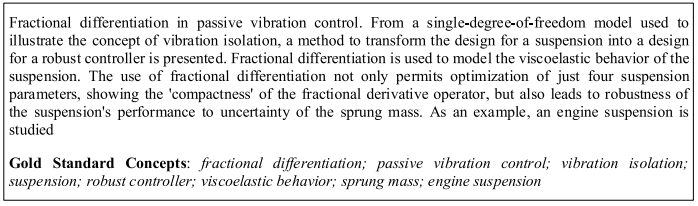
\includegraphics[width = 0.8\linewidth]{fig9.png}
    \caption{\textbf{A sample input text along with the gold standard key concepts from Inspec dataset.}
		\label{fig:f9}}
\end{figure*}

\begin{table*}[!h]
\centering
\caption{\textbf{Output of our proposed technique for the sample document.}}
\label{tab:t10}
\begin{tabular}{|l|l|l|l|} 
\hline
\textbf{No} & \textbf{Candidate} & \textbf{POS} & \textbf{Type}  \\ 
\hline
0  &    \textbf{Fractional differentiation }                           &  ['JJ', 'NN']   & NP    \\
1  &    \textbf{passive vibration control}                             &  ['JJ', 'NN', 'NN']   & NP    \\
2  &    a single-degree-of-freedom model                      &  ['DT', 'JJ', 'NN']   & NP    \\
3  &    the concept                                           &  ['DT', 'NN']   & NP    \\
4  &    \textbf{vibration isolation}                                   &  ['NN', 'NN']   & NP    \\
5  &    the design for a \textbf{suspension}                           &  ['DT', 'NN', 'IN', 'DT', NN']   & NP    \\
6  &    a design for a \textbf{robust controller}                      &  ['DT', 'NN', 'IN', 'DT', 'JJ', NN']   & NP    \\
7  &    \textbf{Fractional differentiation}                            &  ['JJ', 'NN']   & NP    \\
8  &    to model the \textbf{viscoelastic behaviour} of the \textbf{suspension} &  ['TO', 'VB', 'DT', 'JJ', 'NN', 'IN', 'DT', 'JJ', 'NN']   & NP    \\
9  &    the \textbf{viscoelastic behaviour} of the \textbf{suspension}          &  ['DT', 'JJ', 'NN', 'IN', 'DT', 'NN']    & NP    \\
10 &    The use of \textbf{fractional differentiation}                 &  ['DT', 'NN', 'IN', 'JJ', 'NN']   & NP    \\
11 &    showing the of the fractional derivative operator     &  ['VBG', 'DT', 'IN', 'DT', 'JJ', 'JJ', 'NN']   & NP    \\
12 &    the of the fractional derivative operator             &  ['DT', 'IN', 'DT', 'JJ', 'JJ', 'NN']   & NP    \\
13 &    robustness of the \textbf{suspension} performance              &  ['NNS', 'IN', 'DT', 'NN', 'NN']   & NP    \\
14 &    uncertainty of the \textbf{sprung mass}                        &  ['NN', 'IN', 'DT', 'JJ', 'NN']   & NP    \\
15 &    an example                                            &  ['DT', 'NN']   & NP    \\
16 &    an \textbf{engine suspension}                                  &  ['DT', 'NN', 'NN']   & NP    \\
\hline
\end{tabular}
\end{table*}

\begin{enumerate}
   \item{EXPERIMENTAL DETAILS}
	
In this experiment, for each document of the \textit{SemEval-2010} dataset a list of top 15 key concepts were extracted with the hybrid technique. The results from each document were evaluated against the gold standard files provided with the dataset, using the \textit{precision, recall} and \textit{F-measure}. After this, the mean values of the performance measures were computed at each rank position of the extracted keyphrases. The same procedure was adopted to evaluate the results of the TF-IDF and TopicRank.


   \item{RESULTS}
	
In Table \ref{tab:t9} the results of the proposed Hybrid and the existing approaches (i.e. \textit{TF-IDF} and \textit{TopicRank}) are shown. The significant scores achieved in terms of \textit{precision, recall} and \textit{F-measure} are highlighted in bold face. From the results it is evident that the hybrid technique \textit{TF-IDF-Hybrid}achieved significant improvement over the baseline method \textit{TF-IDF} and comparable with TopicRank at cut-off levels of top 5 and top 10 keyphrases. However when extracting top 15 key concepts, the \textit{TF-IDF-Hybrid} achieves maximum \textit{recall} and \textit{F-measure} scores of 19.71\% and 19.49\% respectively.

	\item{DISCUSSION}
	
The impact of using the proposed technique as a foundation for keyphrase extraction can be observed in Figure \ref{fig:f7} and \ref{fig:f8}. The \textit{F-measure} curve of \textit{TfIdfHybrid} show that for each cut-off level of the top N key concepts, the performance of \textit{TF-IDF} improves significantly after replacing the n-gram based technique with the proposed algorithm for candidate feature extraction. The same effect can be seen in the precision-recall curve (i.e. for each percent value of recall the precision improved). Both the figures indicate that the improvement is so obvious and is comparable with the stateof-the- art method TopicRank. This suggests that the proposed technique has the potential to provide firm basis for key concepts identification, especially, when the semantic aspects are considered.
\end{enumerate}


\subsection{ANECDOTAL EVIDENCE}
Here we show an anecdotal evidence for our proposed algorithm. In Figure \ref{fig:f9} a sample input text from \textit{Inspec} dataset
along with the gold standard key concepts is given. The document is processed by our proposed algorithm and the candidate features are extracted. 

Table \ref{tab:t10} shows the output of our proposed technique for the sample document, along with the POS tags and type of the phrase. The phrases from candidate features that match with the gold standard are shown in bold face. We can see that the extracted list contains all the meaningful key concepts from the gold standard, allowing some contextual information around the key concepts, thus achieving 100\% \textit{recall}, 50\% \textit{precision} and 66.67\% \textit{F-measure} score for the sample document.


\section{CONCLUSION}
In this paper, we introduced a novel technique to extract candidate features from unstructured text documents for key concepts identification. In the proposed algorithm, we utilized parsing technique to analyze the sentence structures for  candidate features extraction. The advantage of our technique is that it provides a mechanism to extract a comprehensive and meaningful list of candidate features which carry contextual information for the key concept it represents. This contextual information can be utilized for semantic based information extraction and retrieval. We conducted two kind of  experiments, first to determine the optimal value for the parameter \textit{Context Window} and second, to compare it with the conventional approaches. The experimental results show that the proposed technique achieved the overall significant improvement of 13.51\%, 5.482\% and 13.168\% in terms of \textit{precision, recall} and \textit{F-measure} respectively, and it has the potential to be effectively utilized for the improvement of keyphrase extraction.

In future, we will further improve the candidate feature extraction by integrating it with WordNet to enrich the extracted list of candidate features. We will also investigate the use this technique as a sub task for semantic based indexing and key concepts identification from unstructured text.

\begin{thebibliography}{00}

\bibitem{b1} 
A. Bougouin, F. Boudin, and B. Daille, ‘‘TopicRank: Graph-based topic ranking for keyphrase extraction,’’ in \textit{Proc. Int. Joint Conf. Natural Lang. Process (IJCNLP)}, 2013, pp. 543–551.

\bibitem{b2} 
(2017). \textit{The Stanford Parser.} Accessed: May 2, 2017. [Online]. Available:
https://nlp.stanford.edu/software/lex-parser.html
 

\bibitem{b3}
British Council. (2017). \textit{Learn English.}, Accessed: Dec. 30, 2017.
[Online]. Available: https://learnenglish.britishcouncil.org/en/englishgrammar/clause-phrase-and-sentence/sentence-structure

\bibitem{b4} 
 M.-S. Paukkeri, I. T. Nieminen, M. Pöllä, and T. Honkela, ‘‘A
language-independent approach to keyphrase extraction and evaluation,’’
in \textit{Proc. Coling Companion}, 2008, pp. 83–86.

\bibitem{b5} 
S. R. El-Beltagy and A. Rafea, ‘‘KP-Miner: A keyphrase extraction system
for English and Arabic documents,’’\textit{’ Inf. Syst.}, vol. 34, no. 1, pp. 132–144,
2009.

\bibitem{b6} 
] O. Medelyan, E. Frank, and I. H. Witten, ‘‘Human-competitive tagging
using automatic keyphrase extraction,’’ in\textit{n Proc. Conf. Empirical Methods
Natural Lang. Process.}, vol. 3, 2009, pp. 1318–1327.

\bibitem{b7} 
K. S. Nam, M. Olena, K. Min-Yen, and B. Timothy, ‘‘Semeval-2010 task
5: Automatic keyphrase extraction from scientific articles,’’ in\textit{Proc. 5th
Int. Workshop Semantic Eval.}, 2010, pp. 21–26.

\bibitem{b8} 
] S. N. Kim, O. Medelyan, M.-Y. Kan, and T. Baldwin, ‘‘Automatic
keyphrase extraction from scientific articles,’’ \textit{Lang. Resour. Eval.},vol. 47,
no. 3, pp. 723–742, 2013.


\bibitem{b9} 
S. Danesh, T. Sumner, and J. H. Martin, ‘‘Sgrank: Combining statistical and
graphical methods to improve the state of the art in unsupervised keyphrase
extraction,’’ in\textit{Proc. SEM NAACL-HLT}, 2015, pp. 117–126.

\bibitem{b10}
F. Boudin, ‘‘A comparison of centrality measures for graph-based
keyphrase extraction,’’ in \textit{Proc. Int. Joint Conf. Natural Lang.
Process. (IJCNLP)}, 2013, pp. 834–838.

\bibitem{b11}
Y.-B. Kang, P. D. Haghighi, and F. Burstein, ‘‘CFinder: An intelligent key
concept finder from text for ontology development,’’ \textit{Expert Syst. Appl.},
vol. 41, no. 9, pp. 4494–4504, 2014.

\bibitem{b12}
Z. Liu, W. Huang, Y. Zheng, and M. Sun, ‘‘Automatic keyphrase extraction
via topic decomposition,’’ in \textit{Proc. Conf. Empirical Methods Natural Lang.
Process.}, 2010, pp. 366–376.

\bibitem{b13}
J. Martinez-Romo, L. Araujo, and A. D. Fernandez, ‘‘Semgraph: Extracting keyphrases following a novel semantic graph-based approach,’’
\textit{J. Assoc. Inf. Sci. Technol.}, vol. 67, no. 1, pp. 71–82, 2016.

\bibitem{b14}
N. Teneva and W. Cheng, ‘‘Salience rank: Efficient keyphrase extraction
with topic modeling,’’ in \textit{Proc. 55th Annu. Meeting Assoc. Comput. Linguistics}, vol. 2, 2017, pp. 530–535.

\bibitem{b15}
C. Florescu and C. Caragea, ‘‘Positionrank: An unsupervised approach
to keyphrase extraction from scholarly documents,’’ in \textit{Proc. 55th Annu.
Meeting Assoc. Comput. Linguistics}, vol. 1, 2017, pp. 1105–1115.

\bibitem{b16}
J. Rafiei-Asl and A. Nickabadi, ‘‘TSAKE: A topical and structural automatic keyphrase extractor,’’ \textit{Appl. Soft Comput.}, vol. 58, pp. 620–630,
Sep. 2017.

\bibitem{b17}
A. Hulth, ‘‘Improved automatic keyword extraction given more linguistic
knowledge,’’ in \textit{Proc. Conf. Empirical Methods Natural Lang. Process.},
2003, pp. 216–223.

\bibitem{b18}
F. Boudin and E. Morin, ‘‘Keyphrase extraction for n-best reranking in
multi-sentence compression,’’ in Proc. North Amer. Chapter Assoc. Comput. Linguistics (NAACL), 2013, pp. 1–9.

\bibitem{b19}
R. Barzilay and K. R. McKeown, ‘‘Sentence fusion for multidocument
news summarization,’’ \textit{Comput. Linguistics}, vol. 31, no. 3, pp. 297–328,
2005.
\bibitem{b20}
K. Filippova and M. Strube, ‘‘Sentence fusion via dependency graph
compression,’’ in \textit{Proc. Conf. Empirical Methods Natural Lang. Process.},
2008, pp. 177–185.

\bibitem{b21}
W. You, D. Fontaine, and J.-P. Barthés, ‘‘An automatic keyphrase extraction system for scientific documents,’’ \textit{Knowl. Inf. Syst.}, vol. 34, no. 3,
pp. 691–724, 2013.

\bibitem{b22}
D. Newman, N. Koilada, J. H. Lau, and T. Baldwin, ‘‘Bayesian text
segmentation for index term identification and keyphrase extraction,’’ \textit{in
Proc. COLING}, 2012, pp. 2077–2092.

\bibitem{b23}
C. Huang, Y. Tian, Z. Zhou, C. X. Ling, and T. Huang, ‘‘Keyphrase
extraction using semantic networks structure analysis,’’ in \textit{Proc. 6th Int.
Conf. Data Mining (ICDM)}, Dec. 2006, pp. 275–284.

\bibitem{b24}
F. Wang, Z. Wang, S. Wang, and Z. Li, ‘‘Exploiting description knowledge
for keyphrase extraction,’’ in \textit{Proc. Pacific Rim Int. Conf. Artif. Intell.},
2014, pp. 130–142.

\bibitem{b25}
H. Zheng, Z. Li, S. Wang, Z. Yan, and J. Zhou, ‘‘Aggregating inter-sentence
information to enhance relation extraction,’’ in \textit{Proc. AAAI}, 2016,
pp. 3108–3115.

\bibitem{b26}
K. Bennani-Smires, C. Musat, M. Jaggi, A. Hossmann, and M. Baeriswyl.
(2018). ‘‘EmbedRank: Unsupervised keyphrase extraction using sentence
embeddings.’’ [Online]. Available: https://arxiv.org/abs/1801.04470

\bibitem{b27}
X. Wu, Z. Du, and Y. Guo, ‘‘A visual attention-based keyword extraction
for document classification,’’ \textit{Multimedia Tools Appl.}, vol. 77, no. 19,
pp. 25355–25367, 2018.

\bibitem{b28}
J. Hu, S. Li, Y. Yao, L. Yu, G. Yang, and J. Hu, ‘‘Patent keyword extraction
algorithm based on distributed representation for patent classification,’’
\textit{Entropy}, vol. 20, no. 2, p. 104, 2018.

\bibitem{b29}
D. Klein and C. D. Manning, ‘‘Accurate unlexicalized parsing,’’ in \textit{Proc.
41st Annu. Meeting Assoc. Comput. Linguistics}, 2003, pp. 423–430.

\bibitem{b30}
M. P. Marcus and M. A. Marcinkiewicz, and B. Santorini, ‘‘Building a large
annotated corpus of English: The penn treebank,’’ \textit{Comput. Linguistics},
vol. 19, no. 2, pp. 313–330, 1993.

\bibitem{b31}
L. Marujo, A. Gershman, J. Carbonell, R. Frederking, and J. P. Neto.
(2013). ‘‘Supervised topical key phrase extraction of news stories using
crowdsourcing, light filtering and co-reference normalization.’’ [Online].
Available: https://arxiv.org/abs/1306.4886

\bibitem{b32}
R. Mihalcea and P. Tarau, ‘‘Textrank: Bringing order into text,’’ in \textit{Proc.
Conf. Empirical Methods Natural Lang. Process.}, 2004, pp. 1–8.

\bibitem{b33}
C. J. V. Rijsbergen, Information Retrieval, 2nd ed. Newton, MA, USA:
Butterworth, 1979.

\bibitem{b34}
D. D. Lewis, ‘‘Evaluating and optimizing autonomous text classification
systems,’’ in \textit{Proc. 18th Annu. Int. ACM SIGIR Conf. Res. Develop. Inf.
Retr.}, 1995, pp. 246–254.

\bibitem{b35}
P. D. Turney. (2002). ‘‘Extraction of keyphrases from text: Evaluation of
four algorithms.’’ [Online]. Available: https://arxiv.org/abs/cs/0212014

\bibitem{b36}
F. Boudin, ‘‘Pke: An open source Python-based keyphrase extraction
toolkit,’’ in \textit{Proc. 26th Int. Conf. Comput. Linguistics, Syst. Demonstrations
(COLING)}, 2016, pp. 69–73.

\end{thebibliography}

\begin{IEEEbiography}[{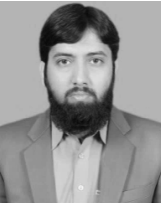
\includegraphics[width=1in,height=1.25in,clip,keepaspectratio]{a1.png}}]{\textbf{MUHAMMAD AMAN}} received the M.S. degree from the University of Science and Technology, Bannu, Pakistan, in 2013. He is currently pursuing the Ph.D. degree with the Department of Computer and Information Sciences, Universiti Teknologi Petronas, Malaysia. The major focus of his work is on the development of intelligent solution for automatic keyphrase identification from text documents that has diverse applications in areas, such as information retrieval, text mining, document summarization, and ontology learning. He is also interested in the analysis of key concepts identification algorithms.
\end{IEEEbiography}

\begin{IEEEbiography}[{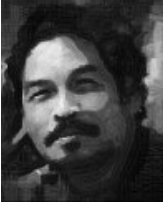
\includegraphics[width=1in,height=1.25in,clip,keepaspectratio]{a2.png}}]{\textbf{ABAS BIN MD SAID}}received the bachelor’s and master’s degrees in applied mathematics from Western Michigan University in 1983 and 1985, respectively, and the Ph.D. degree in IT from Loughborough University in 1997. He is an Associate Professor at the Department of Computer and Information Sciences, Universiti Teknologi Petronas, Malaysia.
\end{IEEEbiography}
\vspace{-8 cm}

\begin{IEEEbiography}[{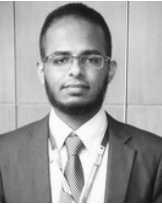
\includegraphics[width=1in,height=1.25in,clip,keepaspectratio]{a3.png}}]{\textbf{SAID JADID ABDUL KADIR}}received the M.Sc. degree in computer science degree from University Teknologi Malaysia in 2012 and the Ph.D. degree in information technology from Universiti Teknology Petronas (UTP), Malaysia. He is currently a Lecturer with the Department of Computer and Information Sciences, UTP.
\end{IEEEbiography}
\vspace{-8 cm}

\begin{IEEEbiography}[{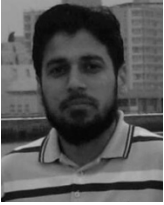
\includegraphics[width=1in,height=1.25in,clip,keepaspectratio]{a4.png}}]{\textbf{ISRAR ULLAH}} received the M.C.S. degree from the Institute of Computing and Information Technology, Gomal University, Pakistan, in 2004, and the M.S. degree in computer science from the National University of Computer and Emerging Sciences, Islamabad, Pakistan, in 2009. He is currently pursuing the Ph.D. degree with Computer Engineering Department, Jeju National University, South Korea. His research work is focused on the application of prediction and optimization algorithms to build IoT-based solutions. His research interests also include analytical modeling, network simulation, and analysis of optimization algorithms.
\end{IEEEbiography}


\EOD

\end{document}
